%=============================================================================
\chapter{The Equations of Moment-Based Radiative Transfer}\label{chap:rt-equations}
%=============================================================================


%-----------------------------------------------------------------------
\section{The Equations of Radiative Transfer and the M1 Closure}
%-----------------------------------------------------------------------

Before we begin with the introduction of the equation of radiative transfer and its associated
equations, let's take a quick aside and note that they contain a plethora of variables and
coefficients. For clarity, an overview of the relevant quantities and coefficients is given in
Table~\ref{tab:rt-variables} along with their respective units.

Returning to the topic at hand, radiation is described by a quantity called the specific intensity
$I_\nu$ \citep[e.g.][]{mihalasFoundationsRadiationHydrodynamics1984,
teyssierTheoreticalAstrophysics2021}, which depends on the frequency $\nu$ of the radiation and is
defined as:

\begin{equation}
	\de E = I_\nu(\x, \mathbf{n}, t) \de A \de \Omega \de \nu \de t \  \label{eq:specific-intensity}
\end{equation}

where $\de E$ is the energy absorbed by the surface element $\de A$ of a detector per unit time
$\de t$ in the frequency range $\de \nu$ coming from a beam projected along the normal of
the surface element $\de A$,\footnote{
The projection along the normal unit vector $\mathbf{n}_A$ of the surface element $\de A$ happens
as a scalar product of the normal unit vector and the direction of propagation of the radiation,
i.e. $\mathbf{n}_A \cdot \mathbf{n}$, which can also be written as an additional factor
$\cos(\theta_A)$, where $\theta_A$ is the angle between $\mathbf{n}$ and $\mathbf{n}_A$. So
eq.~\ref{eq:specific-intensity} may as well be written as
\begin{equation*}
	\de E = I_\nu(\x, \mathbf{n}, t) \cos(\theta_A) \de A \de \Omega \de \nu \de t
\end{equation*} to include the projection explicitly, rather than assume $I_\nu$ is already
projected along the normal vector $\mathbf{n}_A$. This additional factor $\cos(\theta_A)$ is
however the reason why the units of the specific intensity are per radians instead of per
steradians.}
pointing in direction $\mathbf{n}$, and with (solid angle) size $\de \Omega$. $I_\nu$ has units of
erg cm$^{-3}$ rad$^{-1}$ Hz$^{-1}$ s$^{-1}$.


The equation of radiative transfer (RT) is given by:

\begin{align}
    \frac{1}{c} \DELDT{I_\nu} + \mathbf{n} \cdot \nabla I_\nu
        &= \eta_\nu - \alpha_\nu I_\nu \label{eq:RT} \\
        &= \eta_\nu - \sum_j^{\text{photo-absorbing\ species}} \sigma_{j,\nu} n_j I_\nu \ .
\label{eq:RT-sigma}
\end{align}

$\eta_\nu$ is a source function of radiation, i.e. the term describing radiation being added along
the (dimensionless) direction $\mathbf{n}$ due to yet unspecified processes, and has units of erg
cm$^{-3}$ rad$^{-1}$ Hz$^{-1}$ s$^{-1}$, which is the same as the units of the specific intensity
$I_\nu$ per cm. $\alpha_\nu$ is an absorption coefficient, describes how much radiation is being
removed, and has units of cm$^{-1}$. Naturally only as much radiation as is currently present can be
removed, and so the sink term must be proportional to the local specific intensity $I_\nu$.

The equation holds for any photon frequency $\nu$ individually. In eq.~\ref{eq:RT-sigma} we split
the absorption coefficient $\alpha_\nu$ into the sum over the photo-absorbing species $j$, which
throughout this work will only be the main constituents of primordial gas, namely hydrogen, helium,
and singly ionized helium. The photo-absorption process is modeled as binary collisions between
radiation and the photo-absorbing species, where the photo-absorbing species are treated as targets
which collide with the incoming photons. The probability of a collision that leads to a photon being
absorbed is described by an interaction cross section $\sigma_{j,\nu}$, which has units of cm$^2$,
while $n_j$ represents the number density of photo-absorbing species $j$ in cm$^{-3}$.

\begin{table}
\begin{center}
\begin{small}
\begin{tabular}{p{0.32\textwidth} p{0.42\textwidth} p{0.26\textwidth}}


variable  & name & units (cgs) \\[.5em]
%---------------------------------------------------------------------------------------------------
\hline \\

$I_\nu (\x, \mathbf{n}, t)$ &
        specific intensity &
        $[I_\nu] = \frac{\text{erg}}{\text{cm}^2 \text{ rad Hz s}}$ 
\\[.5em]
$u_\nu (\x, \mathbf{n}, t) = \frac{I_\nu}{c}$ &
        radiation energy density &
        $[u_\nu] = \frac{\text{erg}}{\text{cm}^3 \text{ rad Hz}}$
\\[.5em]
$E_\nu (\x, t) = \int_{4 \pi} \frac{I_\nu}{c} \de \Omega$ &
        total energy density &
        $[E_\nu] = \frac{\text{erg}}{\text{cm}^3 \text{ Hz}}$
\\[.5em]
$N_\nu (\x, t) = E_\nu / h$ &
        photon number density &
        $[N_\nu] = \frac{1}{\text{cm}^3 \text{ Hz}}$
\\[.5em]
$E_{rad} (\x, t) = \int_{0}^{\infty} E_\nu \de \nu$ &
        total integrated energy density &
        $[E_{rad}] = \frac{\text{erg}}{\text{cm}^3}$ 
\\[.5em]
$N_{rad} (\x, t) = E_{rad} / h$ &
        integrated photon number density &
        $[N_{rad}] = \frac{1}{\text{cm}^3}$
\\[.5em]
% $J_\nu (\x, t) = \int_{4 \pi} I_\nu \frac{\de \Omega}{4 \pi}
%             = \frac{c}{4 \pi} E_\nu$ &
%             mean radiation specific intensity &
%             $[J_\nu] = \frac{\text{erg}}{\text{cm}^2 \text{ Hz s}}$
% \\[.5em]
$\mathbf{F}_\nu(\x, t) = \int_{4 \pi}  I_\nu \mathbf{n} \de \Omega$ &
        radiation flux &
        $[\mathbf{F}_\nu] = \frac{\text{erg}}{\text{cm}^2 \text{ s Hz}}$
\\[.5em]
$\mathbf{P}_\nu (\x, t) = \frac{\F_\nu}{c^2}$ & 
        radiation momentum density &
        $[\mathbf{P}_\nu] = \frac{\text{erg}}{ \text{cm}^4 \text{ s}^{-1} \text{ Hz}}$
\\[.5em]
$\mathds{P}_\nu (\x, t) = \int_{4 \pi} \frac{I_\nu}{c} \mathbf{n} \otimes \mathbf{n} \de \Omega$ &
        radiation pressure tensor &
        $[\mathds{P}_\nu ] = \frac{\text{erg}}{\text{cm}^3 \text{ Hz}}$ 
         
         
\\
%---------------------------------------------------------------------------------------------------
\hline\\


$\eta_\nu(\x, t)$ &
        source function (of $I_\nu$)&
        $[ \eta_\nu ] = \frac{\text{erg}}{\text{cm}^3 \text{ rad Hz s}}$ 
\\[.5em]
$n(\x, t)$ &
        number density &
        $[ n ] = \text{cm}^{-3}$
\\[.5em]
$\mathcal{J}_\nu(T)$ &
        (specific intensity of a) spectrum &
        $[\mathcal{J}_\nu (T)] = \frac{\text{erg}}{\text{cm}^2 \text{ rad Hz s}}$ 
\\[.5em]
$\Gamma_{\nu, j}$ &
        photoionization rate of species $j$ &
        $[\Gamma] = \text{s}^{-1}$
\\[.5em]
$\mathcal{H}_{\nu,j}$ &
        (photo)heating rate of species $j$ &
        $[\mathcal{H}_{\nu,j}] = \frac{\text{erg}}{s\ cm}^{3}$
\\[.5em]
$\alpha_\nu = \frac{1}{\lambda_\nu} = \rho \kappa_\nu = n \sigma_\nu$ &
        absorption coefficient &
        $[\alpha_\nu] = \text{cm}^{-1}$
\\[.5em]
% $\alpha_E = \frac{\int_0^\infty \alpha_\nu E_\nu \de \nu}{\int_0^\infty E_\nu \de \nu}$ &
% 	 energy mean of abs. coeff. &
% 	 $[\alpha_E] = \text{cm}^{-1}$
% \\[.5em]
% $\alpha_F = \frac{\int_0^\infty \alpha_\nu F_\nu \de \nu}{\int_0^\infty F_\nu \de \nu}$ &
% 	 flux mean of abs. coeff. &
% 	 $[\alpha_F] = \text{cm}^{-1}$
% \\[.5em]
% $j_\nu $ &
%         emission coefficient &
%         $[j_\nu] = \frac{\text{erg}}{\text{cm}^3 \text{rad Hz s}}$
% \\[.5em]
$\lambda_\nu $ &
        mean free path &
        $[\lambda_\nu] = \text{cm}$
\\[.5em]
$\kappa_\nu $ &
        opacity &
        $[\kappa_\nu] = \frac{\text{cm}^2}{\text{g}}$
\\[.5em]
$\tau_\nu(s) = \int_0^s \alpha_\nu(x) \de x$ &
        optical depth &
        $[\tau_\nu] = 1$
\\[.5em]
$\sigma_{j\nu}$ &
        interacton cross section (of species $j$)&
        $[\sigma_{j\nu}] = \text{cm}^2$
\\[.5em]
$\sigma_{ij}^N = \int_{\nu_{i}} N_\nu \ \sigma_{j\nu} \de \nu / \int_{\nu_i} N_\nu \de \nu$ &
        number weighted average cross section &
        $[\sigma_{ij}^N] = \text{cm}^2$
\\[.5em]
$\sigma_{ij}^E = \int_{\nu i} E_\nu \ \sigma_{j\nu} \de \nu / \int_{\nu i} E_\nu \de \nu$ &
        energy weighted average cross section &
        $[\sigma_{ij}^E] = \text{cm}^2$
%

\end{tabular}
\end{small}
\end{center}
\caption{Common quantities appearing in the context of radiative transfer, and their units.}
\label{tab:rt-variables}
\end{table}



% In what follows, we explicitly label the source terms as $\eta_\nu = \eta_\nu^* + \eta_\nu^{rec}$,
% where $\eta^*_\nu$ is the term containing radiation emitted by stars, and $\eta^{rec}_\nu$ is
% radiation stemming from recombination processes, where an ionized atom recombines with a free
% electron and emits a photon in the process.

The equation of radiative transfer already takes the shape of a hyperbolic conservation law, but it
describes how the specific intensity behaves \emph{along a given direction} $\mathbf{n}$. So in
order to solve the equation of radiative transfer for an entire field, we would need to solve it for
all possible directions. This is something we would like to avoid due to the incredible associated
computational expense, and in order to do so, we take the zeroth and first angular moment of
\ref{eq:RT}. Specifically, for the zeroth moment, this means integrating the equation once over all
solid angles $\Omega$, i.e. $\int_\Omega \de \Omega$. For the first moment, the equation is first
multiplied by the direction unit vector $\mathbf{n}$ and then integrated over the entire solid
angle, i.e. $\int_\Omega \mathbf{n} \de \Omega$. Additionally, we make use of the following
quantities:


\begin{align}
	E_\nu (\x, t) &= \int_{4 \pi} \frac{I_\nu}{c} \de \Omega
			&& \text{total energy density }
			&& [E_\nu] = \frac{\text{erg}}{\text{cm}^3 \text{ Hz}}\\
	\Fbf_\nu(\x, t) &= \int_{4 \pi}  I_\nu \mathbf{n} \de \Omega
			&& \text{radiation flux }
			&& [\Fbf_\nu] = \frac{\text{erg}}{\text{cm}^2 \text{ s Hz}}\\
	\mathds{P}_\nu (\x, t) &= \int_{4 \pi} \frac{I_\nu}{c} \mathbf{n} \otimes \mathbf{n} \de \Omega
			&& \text{radiation pressure tensor }
			&& [\mathds{P}_\nu ] = \frac{\text{erg}}{\text{cm}^3 \text{ Hz}}
\end{align}

where $\mathbf{n} \otimes \mathbf{n}$ denotes the outer product, which in components $k$, $l$ gives
%
\begin{align*}
 (\mathbf{n} \otimes \mathbf{n})_{kl} = \mathbf{n}_k \mathbf{n}_l \ .
\end{align*}



This gives us the following equations:


\begin{align}
	\DELDT{E_\nu} + \nabla \cdot \Fbf_\nu &=
		- \sum\limits_{j}^{\absorbers} n_j \sigma_{\nu j} c E_\nu + \dot{E}_\nu
		\label{eq:dEdt-freq} \\
	\DELDT{\Fbf_\nu} + c^2 \ \nabla \cdot \mathds{P}_\nu &=
		- \sum\limits_{j}^{\absorbers} n_j \sigma_{\nu j} c \Fbf_\nu
		\label{eq:dFdt-freq}
\end{align}

which again take the shape of a hyperbolic conservation law with a state vector $\U$, flux tensor
$\F$, and source term $\mathcal{S}$:

\begin{align}
&&
    \DELDT{\U} + \nabla \cdot \F = \mathcal{S}
&&
\\
    \U = \begin{pmatrix}
          E_\nu \\ \Fbf_\nu
         \end{pmatrix}
&&
    \F = \begin{pmatrix}
            \Fbf_\nu \\ c^2 \mathds{P}_\nu
         \end{pmatrix}
&&
    \mathcal{S} = \begin{pmatrix}
		- \sum\limits_{j}^{\absorbers} n_j \sigma_{\nu j} c E_\nu + \dot{E}_\nu \\
		- \sum\limits_{j}^{\absorbers} n_j \sigma_{\nu j} c \Fbf_\nu
         \end{pmatrix}
\end{align}


Note that $E_\nu$ (and $\dot{E}_\nu$) is the radiation energy \emph{density} (and \emph{density}
injection rate) in the frequency interval between frequency $\nu$ and $\nu + \de \nu$ and has
units of $\text{erg / cm}^3 \text{ / Hz}$ (and $\text{erg / cm}^3 \text{ / Hz / s}$).
$\Fbf$ is the radiation flux, and has units of $\text{erg / cm}^2 \text{ / Hz / s}$, i.e.
dimensions of energy per area per frequency per time.

Furthermore, it is assumed that the source term $\dot{E}_\nu$ stems from point sources which radiate
isotropically. This assumption has the consequence that the vector net flux $\Fbf_\nu$ must sum up
to zero, and hence the corresponding source terms in eq.~\ref{eq:dFdt-freq} are zero.
% \footnote{
%     It might be helpful to remember that in the optically thin (free streaming)
%     limit, the relation between radiation flux and energy density is $|\Fbf| = c
%     E$, and in the optically thick (isotropic, LTE) limit, the relation is $|\Fbf|
%     = \frac{1}{3}c E$
% }


To close this set of equations, a model for the pressure tensor $\mathds{P}_\nu$ is necessary. In
the case of the Euler equations, which can also be derived as moments of the Boltzmann equation,
the closure is provided by the equation of state, which relates the pressure, the temperature, and
the internal energy of the gas. For the moments of the equation of radiative transfer, we use the
so-called ``M1 closure'' \citep{levermoreRelatingEddingtonFactors1984} where we describe the
pressure tensor via the Eddington tensor $\mathds{D}_\nu$:

\begin{equation}
	\mathds{P}_\nu = \mathds{D}_\nu E_\nu
\end{equation}

The Eddington tensor is a dimensionless quantity that encapsulates the local radiation field
geometry and its effect in the radiation flux conservation equation. The M1 closure sets the
Eddington tensor to have the form:

\begin{align}
\mathds{D}_\nu &=
    \frac{1- \chi_\nu}{2} \mathds{I} + \frac{3 \chi_\nu - 1}{2} \mathbf{n}_\nu \otimes
    \mathbf{n}_\nu
    \label{eq:eddington-freq} \\
\mathbf{n}_\nu &=
    \frac{\Fbf_\nu}{|\Fbf_\nu|} \\
\chi_\nu &=
    \frac{3 + 4 f_\nu ^2}{5 + 2 \sqrt{4 - 3 f_\nu^2}} \\
f_\nu &=
    \frac{|\Fbf_\nu|}{c E_\nu}
\end{align}

\begin{figure}
 \centering
 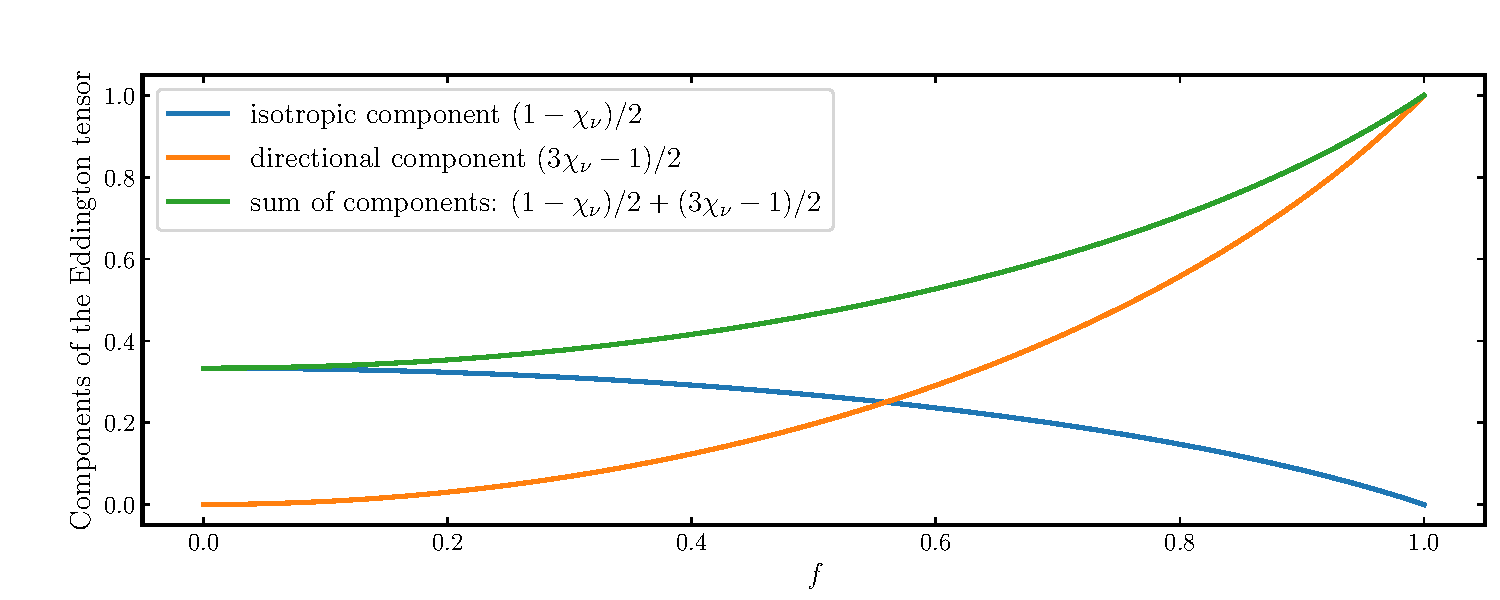
\includegraphics[width=\textwidth]{figures/RHD/chi.pdf}%
 \caption{Components of the Eddington tensor (eq.~\ref{eq:eddington-freq}) depending on the reduced
flux $f_\nu$.}
 \label{fig:eddington-chi}
\end{figure}


The behavior of the Eddington tensor depending on the ``reduced flux'' $f_\nu$ is shown in
Figure~\ref{fig:eddington-chi}. The M1 Closure is an interpolation between extreme cases of fully
isotropic radiation (like blackbody radiation), which is typical for optically thick regimes, and
the free streaming limit which is the case for optically thin regimes. A low value of $f_\nu$
corresponds to predominantly isotropic radiation, while a high value means it is predominantly
flowing in one direction.

This asymptotic behavior can be readily verified, which we shall do now. In the free streaming
limit, the specific intensity of a single point source may be described using a Dirac delta
function:

\begin{equation}
	I_\nu = I_\nu^* \delta(\mathbf{n} - \mathbf{n}_0)
\end{equation}

which gives:

\begin{align}
	\Fbf_\nu &= \int\limits_{4 \pi} I_\nu \mathbf{n} \ \de \Omega = I^*_\nu \mathbf{n}_0 = c E_\nu
\mathbf{n}_0 \\
	\mathds{P}_\nu &= \int\limits_{4 \pi} \frac{I_\nu}{c} \mathbf{n} \otimes \mathbf{n} \de \Omega
=
E_\nu \mathbf{n}_0 \otimes \mathbf{n}_0
\end{align}

and hence

\begin{align}
	|\Fbf_\nu| = c E_\nu && f = \frac{|\Fbf_\nu|}{c E_\nu} = 1 \ .
\end{align}

So for $f_\nu = 1$, we also have $\chi_\nu = 1$, which leads to the correct $\mathds{P}_\nu = E_\nu
\mathbf{n} \otimes \mathbf{n}$ with the M1 Closure.

In the fully isotropic, optically thick case (like blackbody radiation), which constitutes the other
asymptotic case, the pressure tensor is also isotropic, i.e. $\mathds{P}_{11} = \mathds{P}_{22} =
\mathds{P}_{33}$, and using the relation

\begin{align}
	\mathrm{Tr}\ \mathds{P} = \int\limits_{4 \pi} \frac{I_\nu}{c} \de \Omega = E_\nu =
\mathds{P}_{11} + \mathds{P}_{22} + \mathds{P}_{33}
\end{align}

it follows that

\begin{align}
	\mathds{P}_\nu = \frac{E_\nu}{3} \mathds{I} && \mathds{D}_\nu = \frac{1}{3} \mathds{I}
\end{align}

which the M1 Closure correctly gives for $\chi_\nu = 1/3$, or equivalently for $f_\nu = 0$.










%---------------------------------------------------
\section{Interactions Between Radiation and Gas}\label{chap:coupling-to-hydrodynamics}
%---------------------------------------------------


The interactions between gas and radiation manifests in a variety of effects. Radiation can heat
the gas, ionize it, and dissociate molecules. If the radiation field is directed, as opposed to
isotropic, the continuous transfer of momentum from photons onto the gas results in an acceleration
of the gas, which is an effect referred to as ``radiation pressure''. Conversely, the gas can both
absorb and scatter the radiation, as well as emit new radiation. Processes that emit radiation are
for example recombination, which describes a positively charged ion capturing a free electron to
form a neutral atom under emission of a photon, where the photon's energy corresponds to the binding
energy of the newly captured electron. Other examples include the radiation emitted by charged
particles being accelerated, like Bremsstrahlung and synchrotron radiation.

While these interactions can be quite contrived on a microscopic level, their macroscopic
description, particularly in the context of hyperbolic conservation laws, is quite straightforward:
Processes which remove energy and momentum from the radiation fields, i.e. act as sink terms, will
be added as energy and momentum to the gas, i.e. act as source terms in the Euler equations. The
inverse is also true: Gas emitting radiation will remove energy from the gas and add it to the
radiation field, and act as source terms in the moments of the equations of radiative transfer.

In the context of interactions between ionizing radiation and gas, the gas emitting recombination
radiation is particularly common, as it makes an entrance as soon as ionized particles and free
electrons are present. It is then convenient to split up the source term of radiation ($\dot{E}_\nu$
in eq.~\ref{eq:dEdt-freq}) into two individual terms: One containing radiation from radiating
sources like stars, $\dot{E}_\nu^*$, and another that contains the recombination radiation emitted
by the gas, $\dot{E}_\nu^{rec}$, i.e.

\begin{align}
 \dot{E}_\nu = \dot{E}_\nu^* + \dot{E}_\nu^{rec} \ . \label{eq:split-injection-terms}
\end{align}

In this work, I focus only on the heating and ionization of the gas. Specifically, the effects of
radiation pressure and the explicit emission of recombination radiation are omitted. Instead,
recombination is modeled as ``Case B recombination'', where emitted recombination photons are
assumed to be directly re-absorbed by the surroundings, leading to a net lower recombination rate.
This approach is called the ``On The Spot Approximation'' (OTSA), and is generally valid in
optically thick regimes.








%---------------------------------------------------------------
\subsection{Modeling Interactions as Binary Collisions}
%---------------------------------------------------------------

Most of these interactions between gas and radiation can be modeled on a macroscopic scale as
collisions. For example, when a photon and a particle collide, the photon can either be absorbed or
scattered. The scattering can be elastic, and the photon only changes direction, while the photon
energy and the particle's kinetic energy remain constant. This type of scattering is known as
``Thomson scattering''. The scattering can also be inelastic, where the photon and the particle
exchange energies as a consequence of the collision. More precisely, the photon changes both its
direction and its frequency, which is directly proportional to its energy. This process is called
``Compton  Scattering''. Similarly, a photon may be absorbed entirely as a consequence of a
collision.

Binary collisions are commonly described using interaction cross sections $\sigma$, like in
eq.~\ref{eq:RT-sigma}. The basic underlying concept is to have some ``projectiles'' being thrown
with some velocity at some ``targets'' which are at rest. The net collision rates are then
described using probabilities for projectiles and targets to collide. The probability increases
with increasing number of targets, as more targets can be hit. Similarly the probability increases
with increasing number of projectiles for the same reasons. Additionally, the collision \emph{rate}
increases with a higher projectile velocity: A higher velocity means that the projectiles cover a
greater volume over some fixed time interval $\Delta t$. A bigger volume being covered means in turn
that there are more chances for a collision to occur, as the bigger volume would contain more
targets. So some interaction rate $R$ described by the model of binary collisions would need to
satisfy

\begin{align}
    R \propto v_{projectile} \ n_{projectile} \ n_{target}
\end{align}

where $v_{projectile}$ is the projectile velocity, $n_{projectile}$ is the number (density) of
projectiles, and $n_{target}$ is the number (density) of targets. The proportionality can be
resolved into an equality by adding the cross sections $\sigma_{projectile,\ target}$ as the
proportionality constants which encode the interaction probability and have units of cm$^{-2}$:


\begin{align}
    R = \sigma_{projectile,\ target} \ v_{projectile} \ n_{projectile} \ n_{target}
\end{align}









%---------------------------------------------------------------
\subsection{Photo-ionization and Photo-heating Rates}
%---------------------------------------------------------------


In the context of radiative transfer and photo-ionization, the photo-ionization rate $\Gamma_{\nu,
j}$ in units of s$^{-1}$ for photons with frequency $\nu$ and a photo-ionizing particle species $j$
is then given by

\begin{align}
   \DELDT{n_j} = -\Gamma_{\nu, j} \ n_j = - c \ \sigma_{\nu j} \ N_\nu \ n_j
\end{align}

where $N_\nu = E_\nu / (h \nu)$ is the photon number density. Note that the interaction cross
sections are specific to a frequency $\nu$ and the photo-ionizing species $j$ as well. In this work,
I use the analytic fits for the photo-ionization cross sections from
\cite{vernerAtomicDataAstrophysics1996} (via \cite{ramses-rt13}), which are given by

\begin{align}
\sigma(E) &= \sigma_0 F(y) \times 10^{-18} \text{ cm}^2  \label{eq:sigma-parametrizaiton}
\\
F(y) &= \left[(x - 1)^2 + y_w^2 \right] y ^{0.5 P - 5.5} \left( 1 + \sqrt{y / y_a} \right)^{-P}
\\
x &= \frac{E}{E_0} - y_0 \\
y &= \sqrt{x^2 + y_1^2}
\end{align}

where $E$ is the photon energy $E = h \nu$ in eV, and $\sigma_0$, $E_0$, $y_w$, $y_a$, $P$, $y_0$,
and $y_1$ are fitting parameters. The fitting parameter values for hydrogen, helium, and singly
ionized helium are given in Table~\ref{tab:cross-sections}. Figure~\ref{fig:cross-sections} shows
the frequency dependency of the cross sections for these three ionizing species. This fit is valid
for photon energies $E$ which are above the ionization thresholds for the corresponding particle
species. The thresholds are given as frequencies in eqs.~\ref{eq:nuIonHI}-\ref{eq:nuIonHeII}. Below
this threshold, no ionization can take place, and hence the cross sections are zero.



\begin{table}
\centering
\begin{tabular}{l | c c c c c c c }
    & $E_0$ [eV]  & $\sigma_0$ [cm$^2$] & $y_a$ & $P$ & $y_w$ & $y_0$ & $y_1$ \\
\hline\\[-0.5em]
H$^0$  & 0.4298 & 5.475$\times 10^{-14}$ & 32.88 & 2.963 & 0     & 0 & 0 \\
He$^0$ & 13.61  & 9.492$\times 10^{-16}$ & 1.469 & 3.188 & 2.039 & 0.4434 & 2.136 \\
He$^+$ & 1.720  & 1.369$\times 10^{-14}$ & 32.88 & 2.963 & 0     & 0 & 0 \\
 \end{tabular}
\caption{Fitting parameters used for the ionizing cross section parametrizations given in 
eq.~\ref{eq:sigma-parametrizaiton}. The parametrization and these parameters are taken from 
\cite{vernerAtomicDataAstrophysics1996}.}
\label{tab:cross-sections}
\end{table}


\begin{figure}
 \centering
 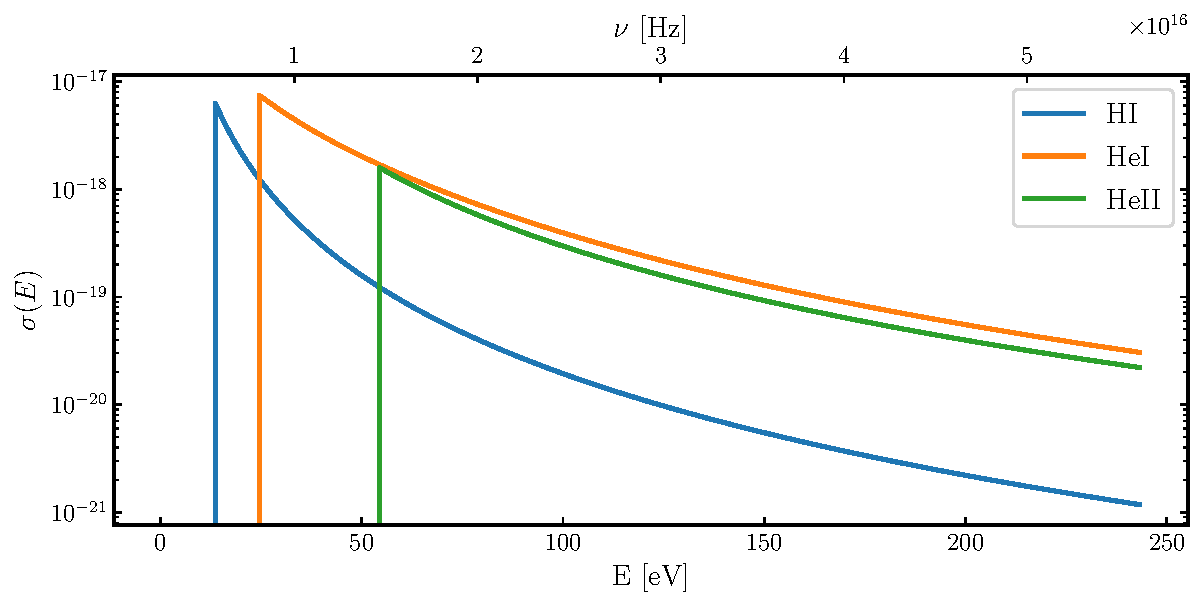
\includegraphics[width=\linewidth]{figures/RHD/cross_sections.pdf}%
\caption{The ionization cross sections parametrizations given by eq.~\ref{eq:sigma-parametrizaiton}.
}
\label{fig:cross-sections}
\end{figure}






Conversely, the rate at which photons are absorbed, i.e. ``destroyed'',  must be equal to the
photo-ionization rate, which means

\begin{align}
\DELDT{N_\nu} &= -c \ \sigma_{\nu j} n_j N_\nu
\end{align}

or in terms of photon energy density $E_\nu$:

\begin{align}
\DELDT{E_\nu} &= h \ \nu \DELDT{N_\nu}  = -h\ \nu \ c \ \sigma_{\nu j} n_j N_\nu
\end{align}



Finally, the photo-heating rate is modeled as the rate of excess energy absorbed by the gas during
photo-ionizing collisions. To ionize an atom, the photons must carry a minimal energy corresponding to the ionizing frequency  $\nu_{ion,j}$ for a photo-ionizing species $j$. In the case of hydrogen and helium, their values are

\begin{align}
    \nu_{\text{ion,HI}} &= 2.179 \times 10^{-11} \text{ erg} = 13.60 \text{ eV} \label{eq:nuIonHI}\\
    \nu_{\text{ion,HeI}} &= 3.940 \times 10^{-11} \text{ erg} = 24.59 \text{ eV}
\label{eq:nuIonHeI}\\
    \nu_{\text{ion,HeII}} &= 8.719 \times 10^{-11} \text{ erg} = 54.42 \text{ eV}
\label{eq:nuIonHeII}
\end{align}

All excess energy is added to the gas in the form of internal energy, and the heating rate
$\mathcal{H}$ (in units of erg cm$^{-3}$ s$^{-1}$ ) for photons of some frequency $\nu$ and some
photo-ionizing species $j$ is described by

\begin{align}
\mathcal{H}_{\nu, j} = (h \nu - h \nu_{ion,j}) \ c \ \sigma_{\nu j} \ n_j \ N_\nu
\end{align}
